\documentclass[14pt,handout]{beamer}
%aspectratio=169
\usepackage[utf8]{inputenc}
\usepackage[T1]{fontenc}
\usepackage[magyar]{babel}
\usetheme{default}
\usepackage{subcaption} %subfigure

%\usepackage{pgfpages}
%\pgfpagesuselayout{4 on 1}[a4paper,border shrink=5mm]
% print with space for notes
%\usepackage{handoutWithNotes} 
% put 3 slides on 1 page with space for notes
%\pgfpagesuselayout{3 on 1 with notes}[a4paper, border shrink=5mm]

%oldalszam
\addtobeamertemplate{navigation symbols}{}{%
	\usebeamerfont{footline}%
	\usebeamercolor[fg]{footline}%
	\hspace{1em}%
	\insertframenumber/\inserttotalframenumber
}

%\usepackage{enumitem} %settings of itemize, e.g. itemsep


\title{Korszerű fűtési rendszerek szabályozása}
\author{Gyulai László}
%\institute{Szakdolgozat bemutatás}
\date{2019. január 7.}

\newcommand\Fontvi{\fontsize{6}{7.2}\selectfont}


\usepackage{graphicx}
\usepackage{tikz}
\usetikzlibrary{mindmap,trees}
\usepackage{verbatim}

%\begin{document}
%	\pagestyle{empty}
	
	\begin{comment}
	:Title: Computer science mindmap
	:Tags: Manual, Mindmap
	
	Version 1.09 of PGF/TikZ added a library for drawing mindmaps. Here's an example
	from the manual. 
	
	| Author: Till Tantau
	| Source: The PGF/TikZ manual
	
	\end{comment}
	%\end{document}

\begin{document}
	
	\frame{\titlepage}
%\begin{frame}{Bevezető}
%
%%[shrink=-25]
%    \begin{itemize}
%        \item Témaválasztás szempontjai
%        \pause
%        \setlength{\itemsep}{6pt}
%        \begin{itemize}
%            \item szabályozástechnikai vonatkozás
%            \item gyakorlati haszon, piaci igény 
%        \end{itemize}
%    	\pause
%    	\item \underline{Korszerű fűtési rendszerek szabályozása}
%    	\pause
%        \begin{itemize}
%            \setlength{\itemsep}{3pt}
%        	\item a fenti kívánalmaknak megfelel
%        	        	
%	    	\item a témában érintett szakterületek:
%	    	\pause
%	        \begin{itemize}
%	            \item Épületgépészet
%	            \item Szabályozástechnika
%	            \item Jogszabályok, pénzügy és marketing 
%	            %környezetgazdaságtan
%	        \end{itemize}
%        \end{itemize}
%    \end{itemize}
%
%\end{frame}

\begin{frame}{A munka célja}
\begin{itemize}
	\setlength{\itemsep}{6pt}
	\item Szabályozástechnikai tudás elmélyítése \pause
	\item Kutatási eredmények megismerése \pause
	\item Törekvés a piacképességre is	
\end{itemize}
\end{frame}




%\begin{frame}{Műszaki tartalom}
%\Fontvi
%\centering
%\begin{tikzpicture}[thick,scale=0.7, every node/.style={scale=0.7}]
%\path[mindmap,concept color=black,text=white]
%node[concept] {\normalsize Termékfejlesztés}
%[clockwise from=-30]
%child[concept color=green!50!black] {
%	node[concept] {Tudás-\\vezérelt\\ötlet}
%	[clockwise from=0]
%	child { node[concept] {épületfizika} }
%	child {
%		node[concept] {szabályozástechnika}
%		[clockwise from=-45, level 3 concept/.append style={sibling angle=50, thick,scale=1.1}]
%		child { node[concept] {MIMO\\rendszerek} }
%		child { node[concept, scale=1.2] { \scalebox{0.9}{prediktív}\\ \scalebox{0.9}{szabályozás}} }
%	}
%	%child { node[concept] {pro\-gramming languages} }
%}  
%child[concept color=blue] {
%	node[concept] {applied}
%	%	[clockwise from=-30]
%	%	child { node[concept] {databases} }
%	%	child { node[concept] {WWW} }
%}
%child[concept color=red] {
%	node[concept] {Piacvezérelt\\ ötlet}
%	[clockwise from=-90]
%	child { node[concept] {törvényi \\ előírások} }
%	child { node[concept] {piaci \\ igények} }
%};
%\end{tikzpicture}
%\end{frame}
%
%
%
%



\begin{frame}{Műszaki tartalom}
\Fontvi
\centering
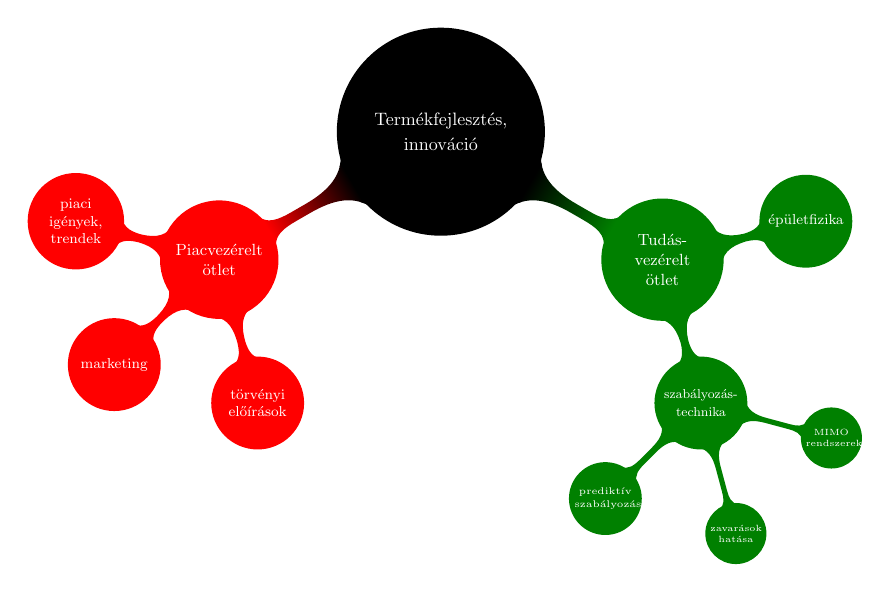
\begin{tikzpicture}[thick,scale=0.65, every node/.style={scale=0.65}]
\path[mindmap,concept color=black,text=white]
node[concept] {\normalsize Termékfejlesztés,\\innováció}
[counterclockwise from=210, level 1 concept/.append style={sibling angle=120}]

child[concept color=red] {
node[concept] {Piacvezérelt\\ ötlet}
[clockwise from=-75, level 2 concept/.append style={sibling angle=60}]
child { node[concept] {törvényi \\ előírások} }
child { node[concept] {marketing} }
child { node[concept] {piaci \\ igények,\\trendek} }
}
child[concept color=green!50!black] {
node[concept] {Tudás-\\vezérelt\\ötlet}
[clockwise from=15, level 2 concept/.append style={sibling angle=90}]
child { node[concept] {épületfizika} }
child {
	node[concept] {\scalebox{0.9}{szabályozás-}\\ \scalebox{0.9}{technika}}
	[clockwise from=-15, level 3 concept/.append style={sibling angle=60, thick,scale=1.1}]
	child { node[concept] {MIMO\\rendszerek} }
	child { node[concept] {zavarások\\hatása} }
	child { node[concept, scale=1.2] { \scalebox{0.9}{prediktív}\\ \scalebox{0.9}{szabályozás}} }
}
%child { node[concept] {pro\-gramming languages} }
};
\end{tikzpicture}
\end{frame}

\begin{frame}{Piacvezérelt termékfejlesztés}

Mire van igény a piacon?
\pause

\begin{itemize}
	\setlength{\itemsep}{7pt}
	\item Van egy problémakör:
	\begin{itemize}
		\item energiahatékonyság (törvényi megfelelőség)
		\item nagy kibocsátás
		\item magas költségek
		\item diszkomfort
	\end{itemize}
	\pause
	
	\item Megoldási lehetőség:
	\begin{itemize}
		\item egy korszerű fűtésszabályozás,\\
		ami teljesíti a követelményeket?
		%\item intelligens otthonok (marketinggel fűszerezve)
	\end{itemize}
\end{itemize}
\end{frame}

\begin{frame}{Tudásalapú termékfejlesztés}

Mit szeretnék csinálni?
\pause
\vspace{6pt}

\begin{itemize}
	\setlength{\itemsep}{12pt}
	\item Szabályozástechnika (analízis és tervezés):
	\begin{itemize}
		\item MISO rendszer, bizonytalansággal
		\item mérhető vagy becsülhető zavarások
		\item prediktív szabályozás
	\end{itemize}
	\pause

	\item Fejlesztési lehetőség:
	\begin{itemize}
		\item egy korszerű fűtésszabályozás, \\
		amivel a fentiek vizsgálhatók, szemléltethetők?
		%\item intelligens otthonok (marketinggel fűszerezve)
	\end{itemize}
\end{itemize}
\end{frame}

\begin{frame}{A kiválasztott irány}

Szabályozástechnikai feladat:

\begin{itemize}
	\item helyiségenkénti hőmérsékletszabályozás,
	\item radiátoros és padlófűtéssel
\end{itemize}
\vspace{6pt}

Ehhez szükséges:

\begin{itemize}
	\item szakaszmodell
	\item modell-prediktív szabályozó
\end{itemize}


\end{frame}


\begin{frame}{Modell struktúrája}

Simulink modell Simscape elemekkel:
\begin{itemize}
	\item RC-hálózat
	\item paraméterezehető az \\ energetikai tanúsítványból
\end{itemize}

\begin{figure}
	\centering
	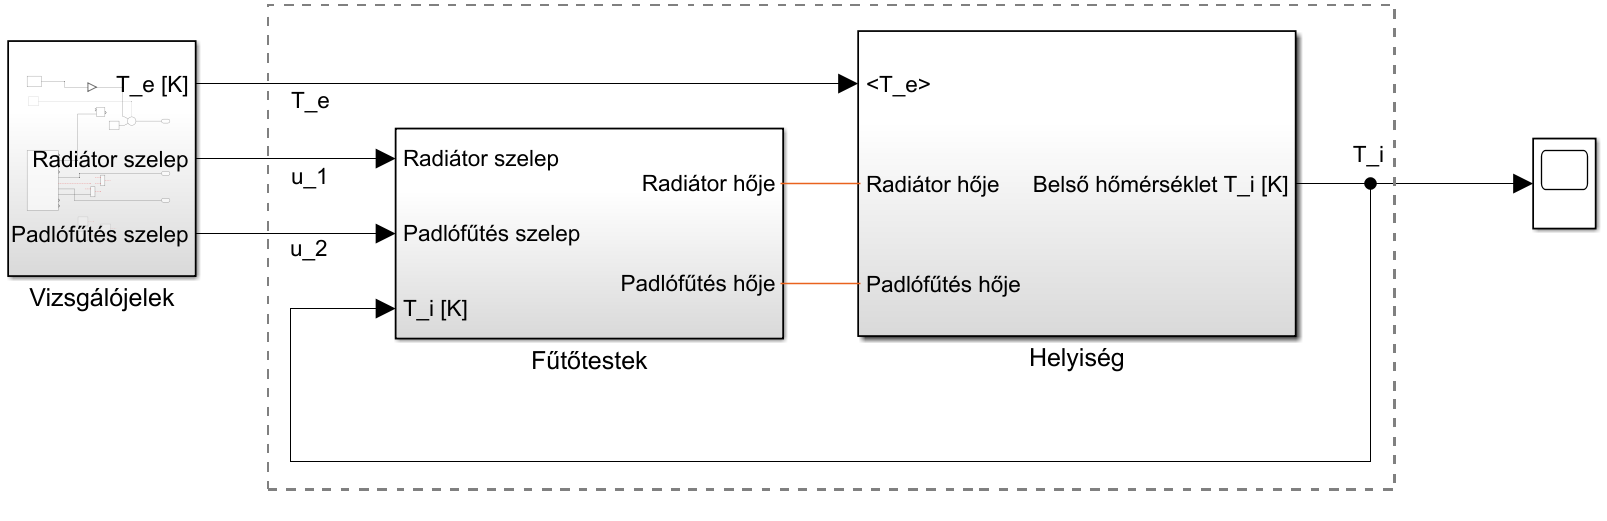
\includegraphics[width=\textwidth]{picture/simulink-network-minimalist-layout.PNG}	
\end{figure}
\end{frame}


\begin{frame}{Tervezés lépései}
\Fontvi
\centering
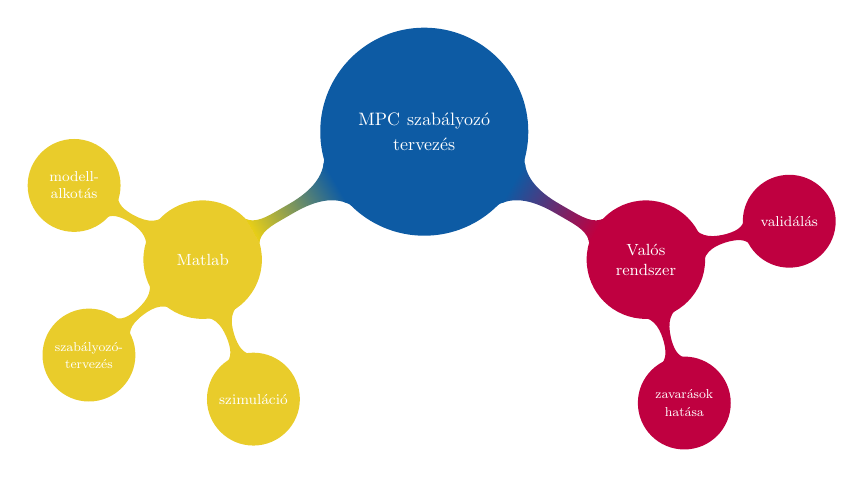
\begin{tikzpicture}[thick,scale=0.65, every node/.style={scale=0.65}]
%\tikzset{level 1 concept/.append style={level distance = 90mm, scale=0.5}}
\path[mindmap,concept color=blue!66!green!90!gray,text=white]
node[concept] {\normalsize MPC szabályozó\\tervezés}
[counterclockwise from=210, level 1 concept/.append style={node distance=6cm,sibling angle=120}]

child[concept color=yellow!80!gray!90!red] {
	node[concept] {Matlab}
	[clockwise from=-70, level 2 concept/.append style={sibling angle=70}]
	child { node[concept] {szimuláció} }
	%child { node[concept] {energetikai\\tanúsítvány} }
	child { node[concept] {\scalebox{0.9}{szabályozó-}\\ \scalebox{0.9}{tervezés}} }
	child { node[concept] {modell-\\alkotás} }
}
child[concept color=blue!25!red] {
	node[concept] {Valós rendszer}
	[clockwise from=15, level 2 concept/.append style={sibling angle=90}]
	child { node[concept] {validálás} }
	child {
		node[concept] {\scalebox{0.9}{zavarások}\\ \scalebox{0.9}{hatása}}
		[clockwise from=-15, level 3 concept/.append style={sibling angle=60, thick,scale=1.1}]
		%child { node[concept] {historikus\\adatok} }
		%child { node[concept, scale=1.2] { \scalebox{0.9}{prediktív}\\ \scalebox{0.9}{szabályozás}} }
	}
	%child { node[concept] {pro\-gramming languages} }
};
\end{tikzpicture}
\end{frame}





%\begin{frame}{Szimuláció, modellalkotás}
%
%A modell nagyon részletesen szerepel a dolgozatban, elvi újdonságot nem tartlalmaz (RC-hálózat) és a szabályozás rész érdekesebb, azzal foglalkoznék.
%
%Tervezés szimulációval.
%\end{frame}

%\begin{frame}{Tervezés lépései}
%
%Szimuláció:
%\begin{itemize}
%	\item valós rendszer modelljének paraméterezése
%	\item modell identifikáció
%	\item szabályozás tervezése, validálása
%\end{itemize}
%\vspace{6pt}
%
%Valós rendszerre:
%\begin{itemize}
%	\item a tervezett szabályozó kipróbálása
%	\item finomítás
%\end{itemize}
%
%\end{frame}



%\begin{frame}{MPC szabályozás}
%
%Publikációk alapján a leggyakoribb korszerű szabályozó
%
%\begin{itemize}
%	\setlength{\itemsep}{12pt}
%	\item Modellalapú működés
%	\begin{itemize}
%		\item fűtési rendszer (helyiség + fűtőtest)
%		\item prediktív szabályozás
%	\end{itemize}
%	\item Követelményei:
%	\begin{itemize}
%		\item radiátorszelep
%		\item hőmérő
%	\end{itemize}
%\end{itemize}
%\end{frame}



\begin{frame}{MPC tervezés}

\begin{itemize}
\item tervezéshez lineáris modell szükséges
\item szakasz nemlinearitással
\end{itemize}

\begin{figure}
	\centering
	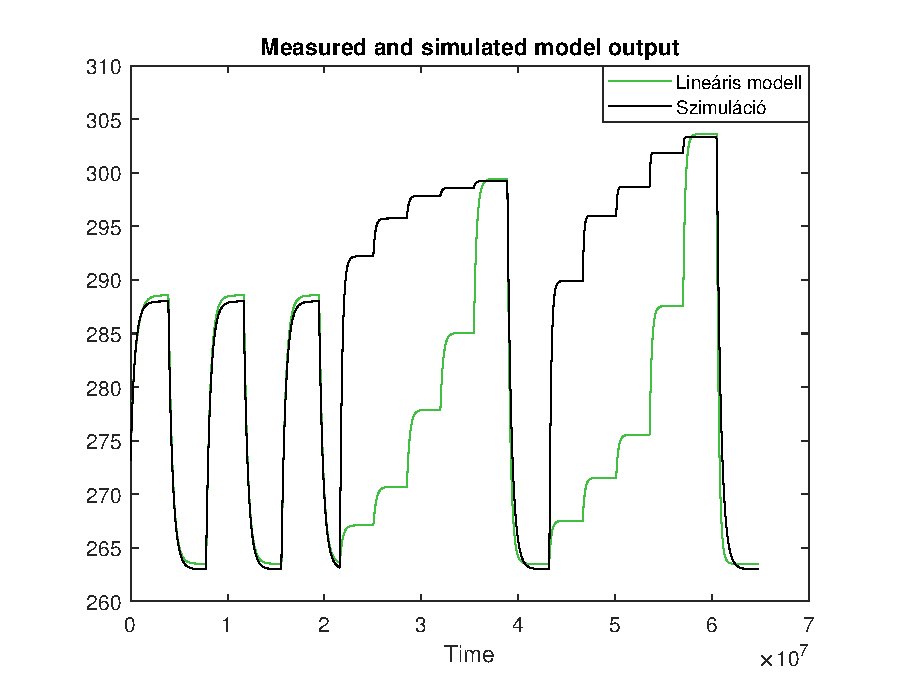
\includegraphics[width=0.8\textwidth]{picture/identModelOutputMatch.eps}	
\end{figure}

\end{frame}


\begin{frame}{MPC tervezés}

\begin{itemize}
\item Simscape modell
\item szabályozás gyengeségei
\end{itemize}

\begin{figure}
\centering
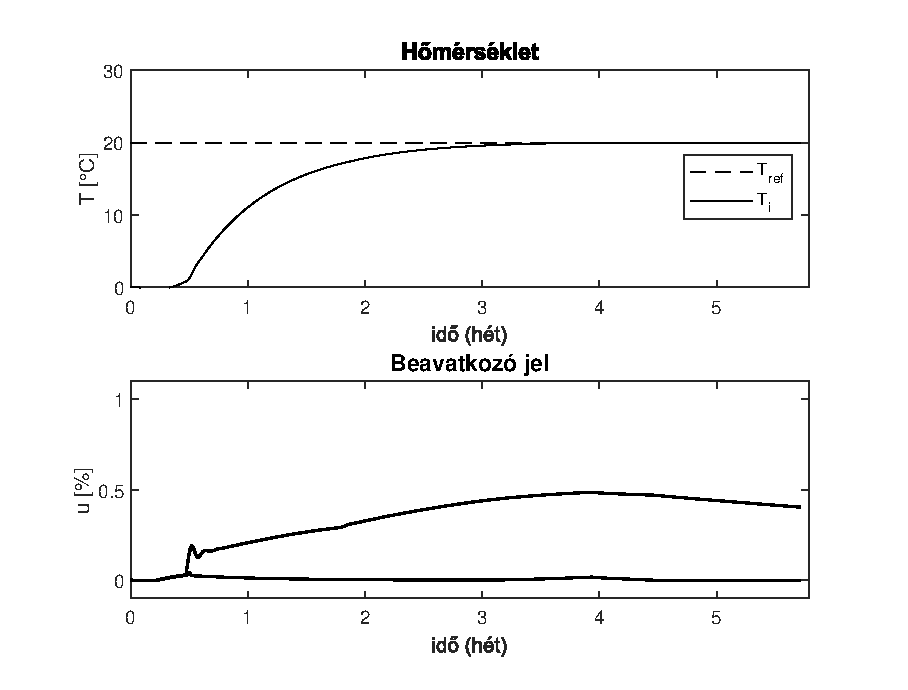
\includegraphics[width=0.8\textwidth]{picture/mpc.eps}	
\end{figure}

\end{frame}

\begin{frame}{MPC tesztrendszer}

%Tesztrendszer, hogy ne csak szimuláció legyen
%\vspace{20pt}

Segít megérteni a szabályozás működését:
\begin{itemize}
	\item tervezés továbbra is részben szimulációval
	\item teszt a gyakorlatban
	\item fűtés izzóval
	\item hőtároló anyagok használata
%	\item Működik a modellre tervezett szabályozás?
%	\item Mennyi idő a funkciók fejlesztése?
%	\item Segít megérteni a szabályozást
\end{itemize}


\begin{figure}
	\begin{subfigure}[t]{0.45\textwidth}
		%			\centering
		%			% trim={<left> <lower> <right> <upper>}
		%			\includegraphics[trim={0cm 11cm 0 0},clip,width=8cm]{figures/hw/sindyCANwirecolor}
		\centering
		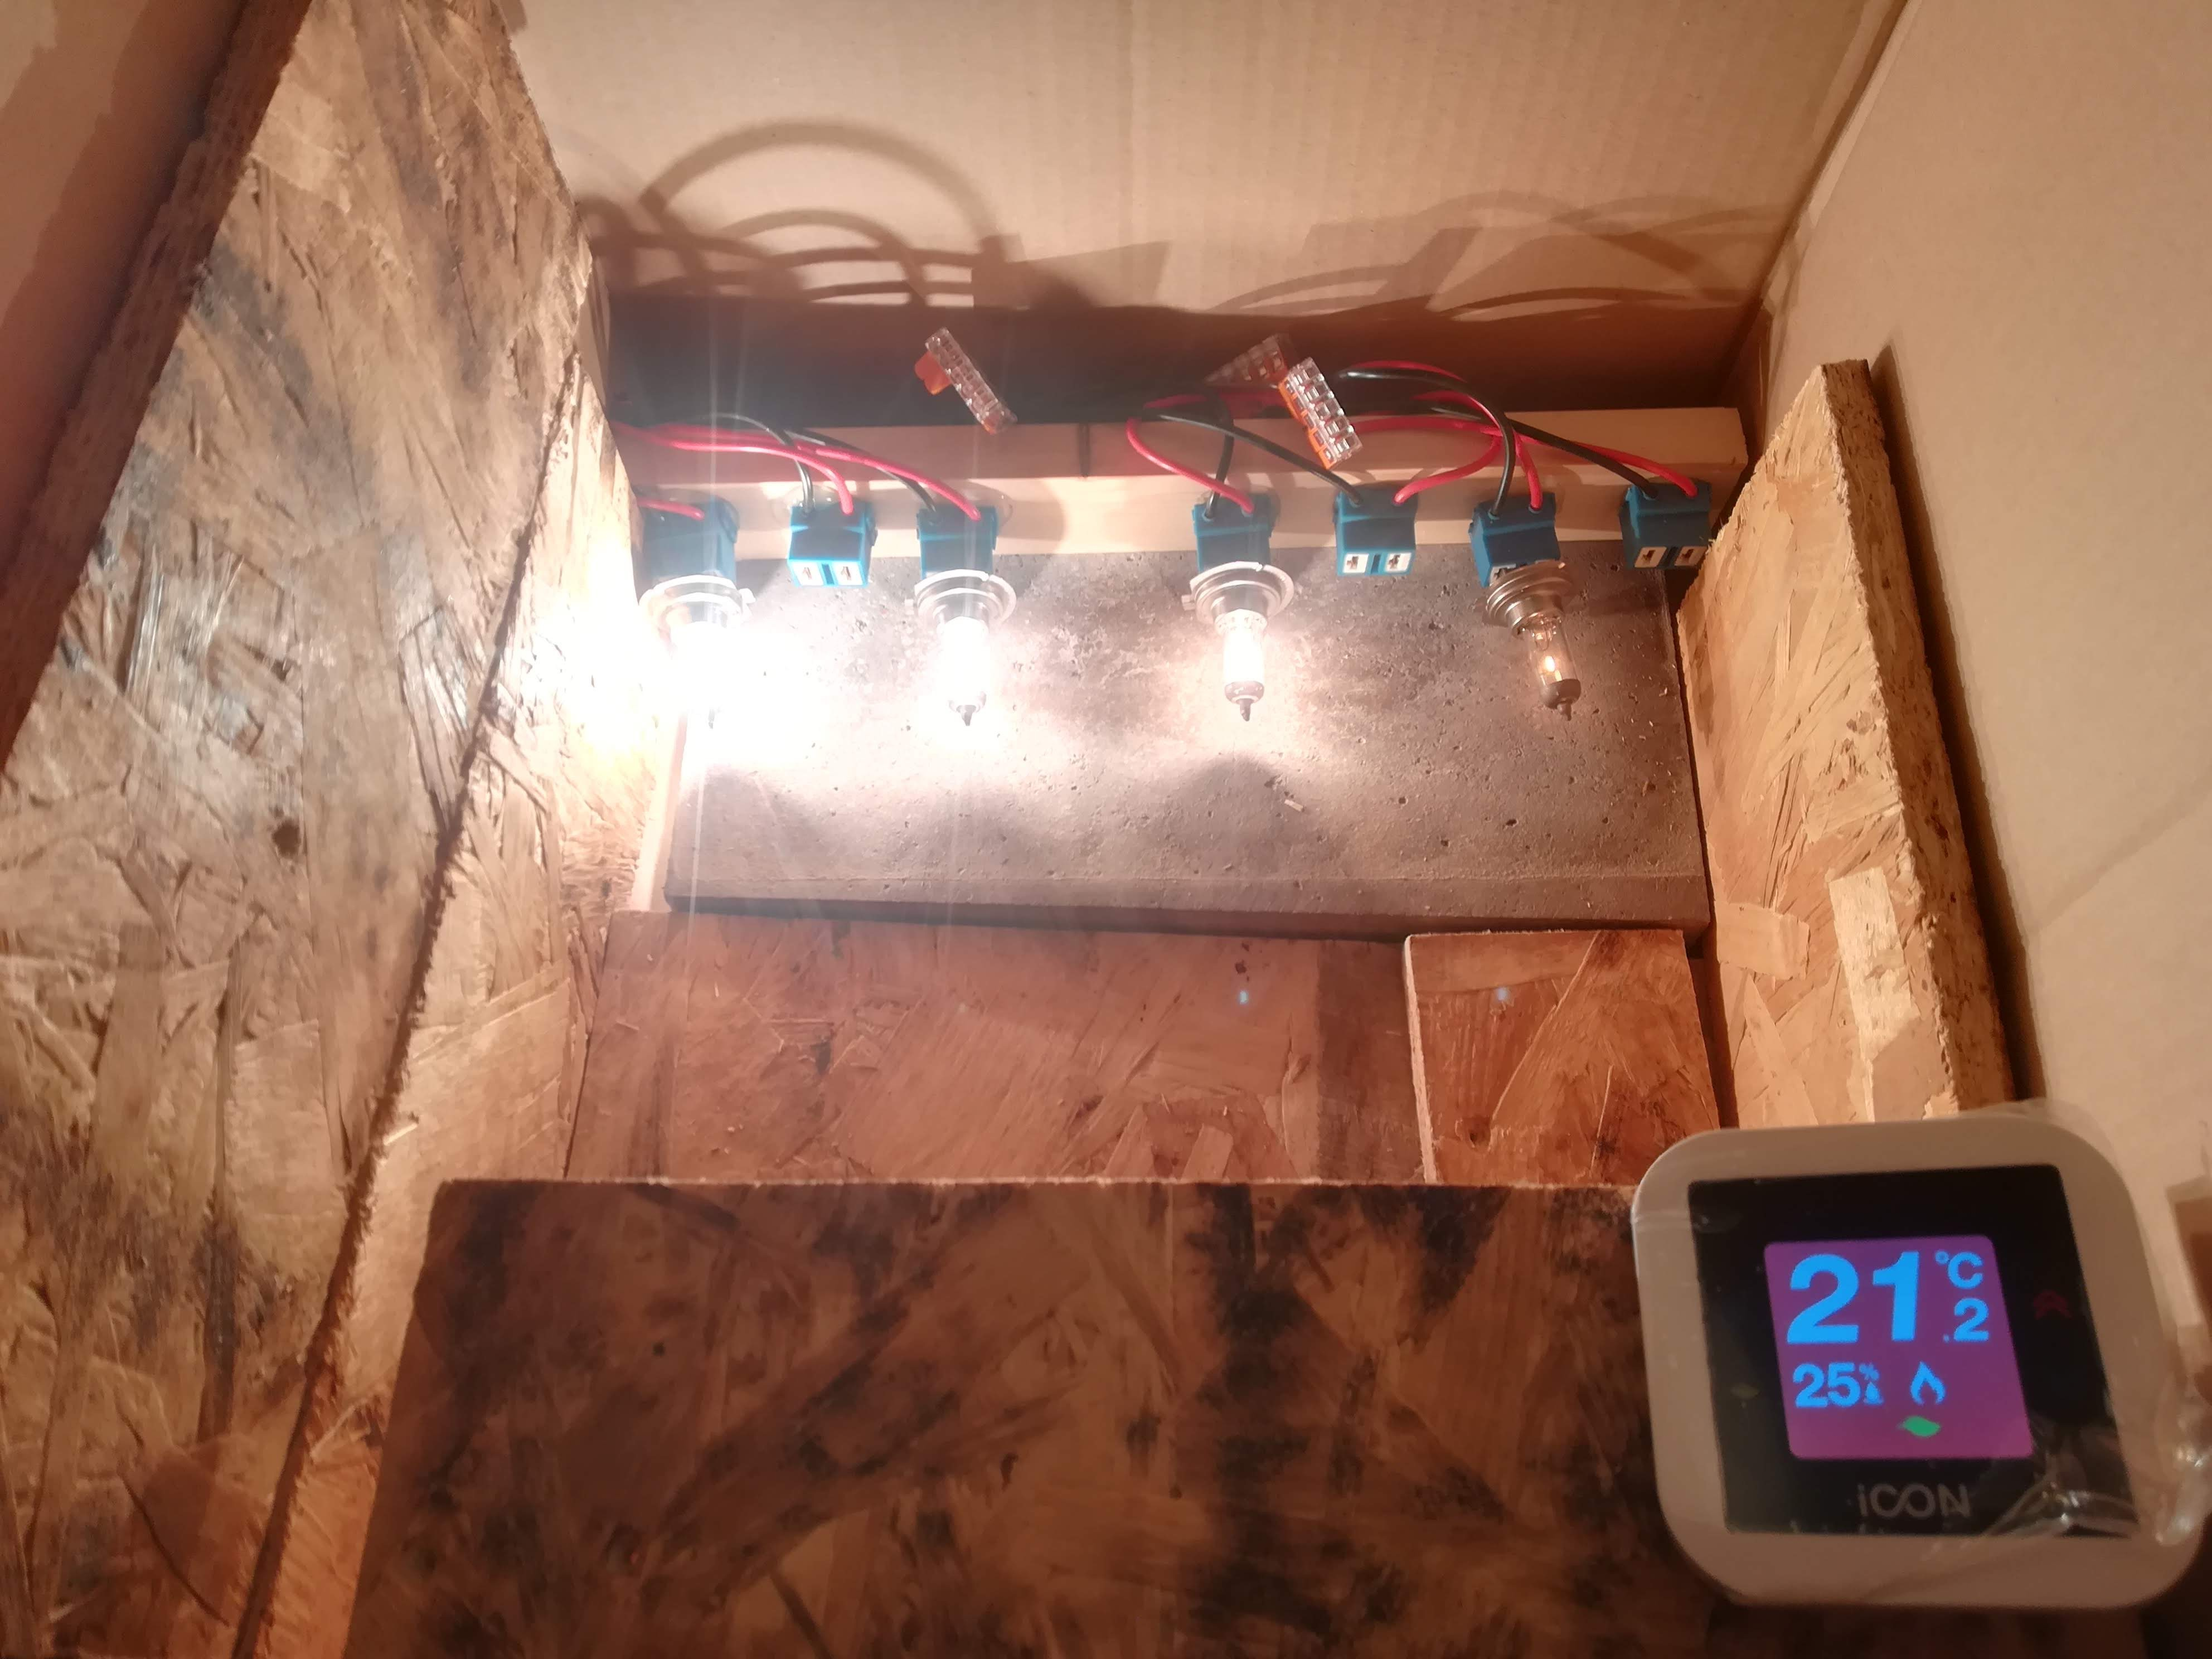
\includegraphics[width=\textwidth]{picture/inside2.jpg}	
	\end{subfigure}
	~
	\begin{subfigure}[t]{0.45\textwidth}
		\centering
		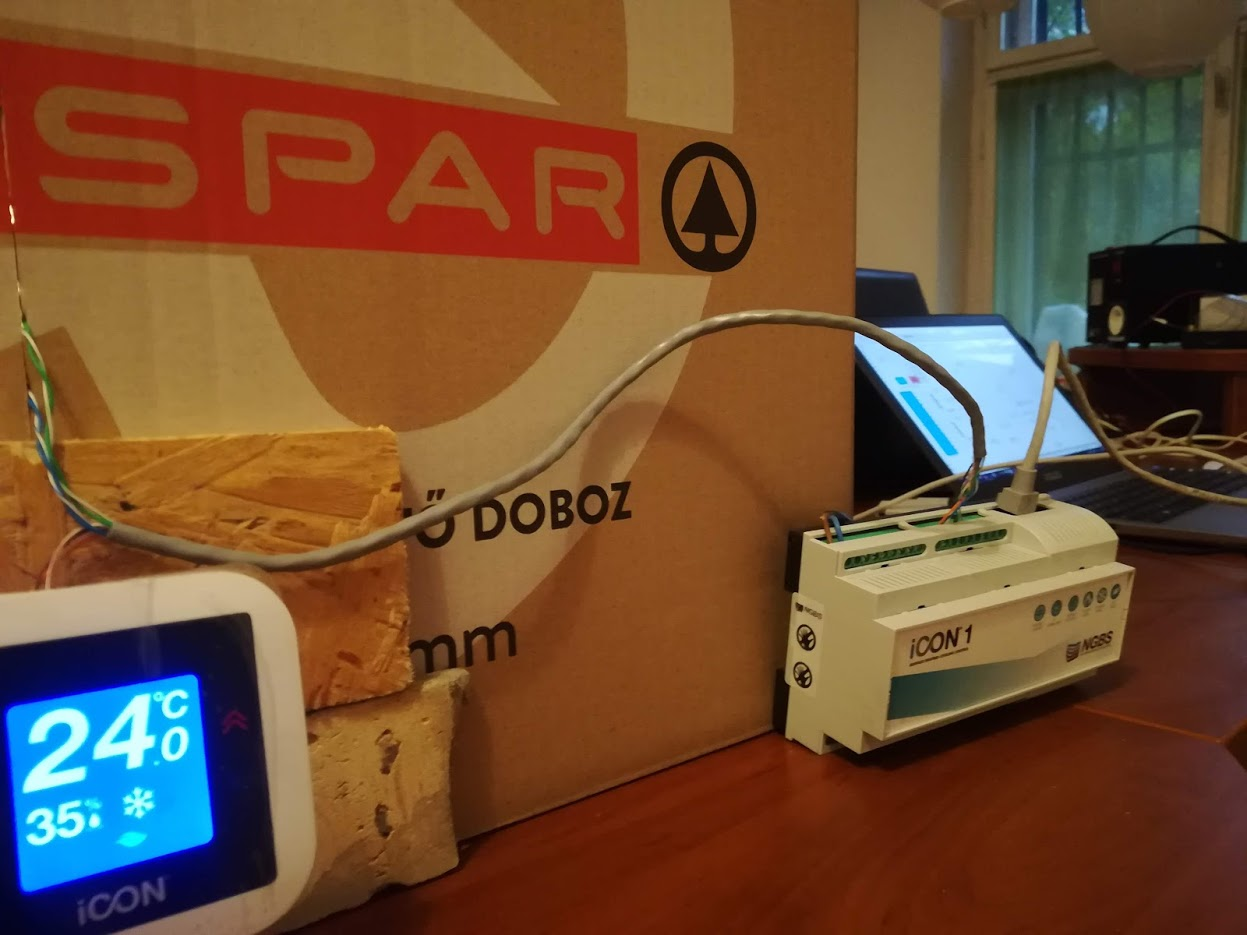
\includegraphics[width=\textwidth]{picture/outside.jpg}	
	\end{subfigure}
\end{figure}

\end{frame}

\begin{frame}{MPC tervezés}

\begin{itemize}
	\item predikciós horizont, korlátok
	\item költségfüggvény súlyai
	\item zavarás hatása
\end{itemize}

\begin{figure}
	\centering
	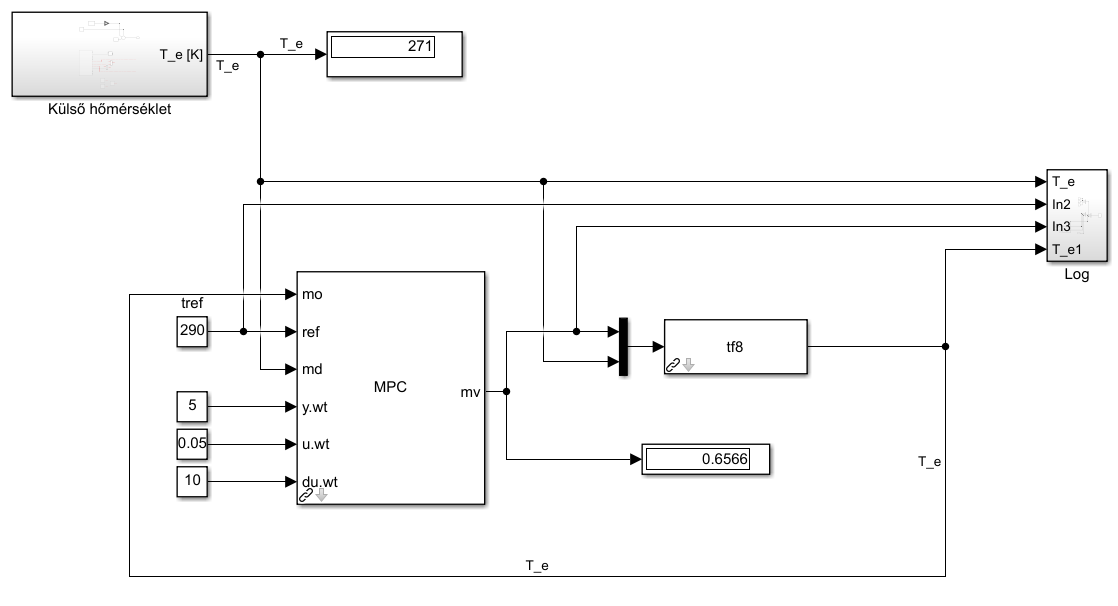
\includegraphics[width=0.9\textwidth]{picture/3-simModel.PNG}	
\end{figure}

\end{frame}


\begin{frame}{MPC költségfüggvénye}

Súlyozás - követelmény alapján

\begin{figure}
	\begin{subfigure}[t]{0.35\textwidth}
		%			\centering
		%			% trim={<left> <lower> <right> <upper>}
		%			\includegraphics[trim={0cm 11cm 0 0},clip,width=8cm]{figures/hw/sindyCANwirecolor}
		\centering
		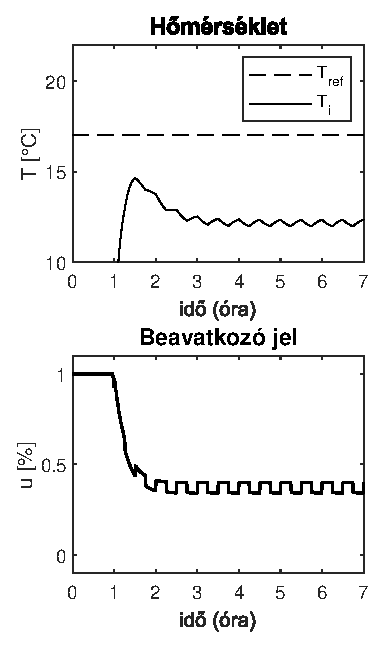
\includegraphics[width=\textwidth]{picture/mpc-wu-20.eps}
		\caption{$w_{u}$=20}	
	\end{subfigure}
	~
	\begin{subfigure}[t]{0.35\textwidth}
		\centering
		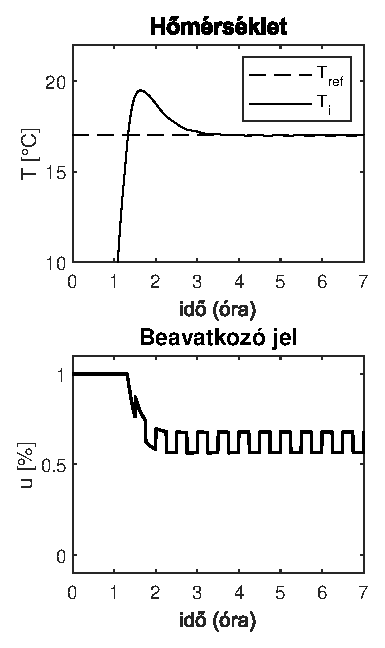
\includegraphics[width=\textwidth]{picture/mpc-wu-005.eps}	
		\caption{$w_{u}$=0.05}	
	\end{subfigure}
\end{figure}

\end{frame}

\begin{frame}{Beavatkozójel változásának költsége}


\begin{figure}
\begin{subfigure}[t]{0.35\textwidth}
	%			\centering
	%			% trim={<left> <lower> <right> <upper>}
	%			\includegraphics[trim={0cm 11cm 0 0},clip,width=8cm]{figures/hw/sindyCANwirecolor}
	\centering
	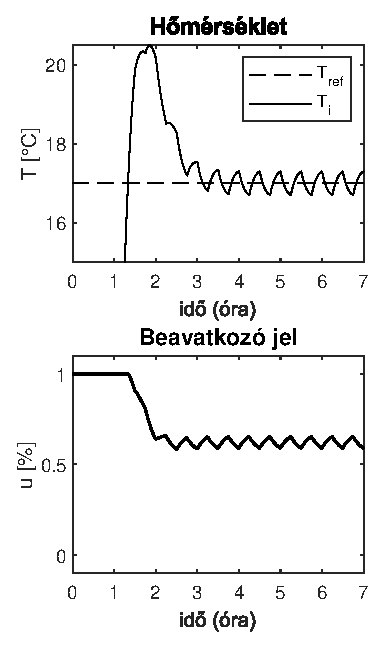
\includegraphics[width=\textwidth]{picture/mpc-wdu-100.eps}
	\caption{$w_{\Delta u}$=100}	
\end{subfigure}
~
\begin{subfigure}[t]{0.35\textwidth}
	\centering
	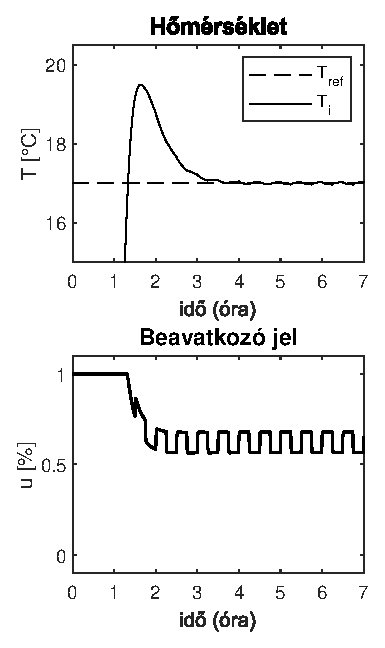
\includegraphics[width=\textwidth]{picture/mpc-wdu-10.eps}	
	\caption{$w_{\Delta u}$=10}	
\end{subfigure}
\end{figure}

\end{frame}





\begin{frame}{Tesztrendszer viselkedése}

Mérési eredmények:

\begin{figure}
	\centering
	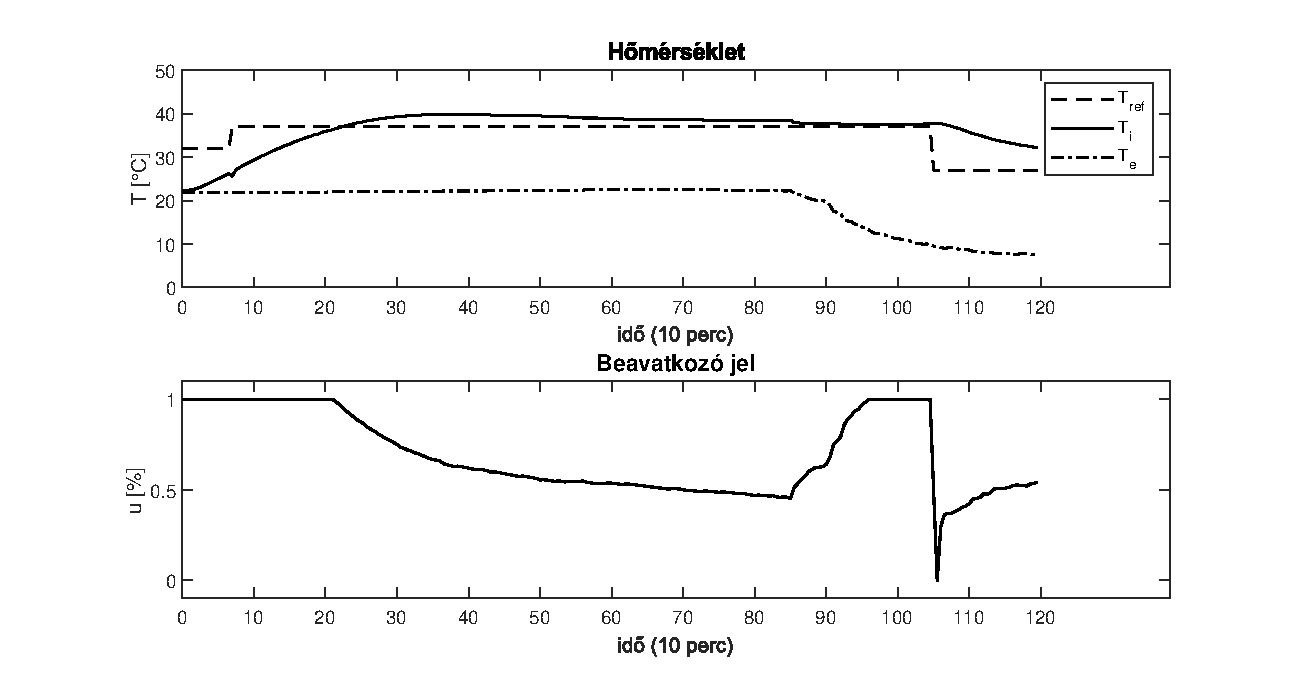
\includegraphics[width=\textwidth]{picture/4-step.eps}	
\end{figure}

\end{frame}



\begin{frame}{Értékelés szempontjai}

	Referenciakövetés:
	\begin{itemize}
		\item megnövekedett komfort
		\item zavarelnyomás
	\end{itemize}
	\vspace{6pt}
	
	Energiamegtakarítás:
	\begin{itemize}
		\item beavatkozás forintosított költségei
		\item integráció okos otthonba
	\end{itemize}
\end{frame}

%\begin{frame}{További feladatok}
%
%	Szabályozó:
%	\begin{itemize}
%		\item megnövekedett komfort
%		\item zavarelnyomás
%	\end{itemize}
%	\vspace{6pt}
%	
%	Energiamegtakarítás:
%	\begin{itemize}
%		\item beavatkozás forintosított költségei
%	\end{itemize}
%
%\end{frame}

\begin{frame}{}
	\begin{center}
		\vspace{18pt}
		\large
		{\usebeamercolor[fg]{structure} 
			Köszönöm a figyelmet, \\
			várom a kérdéseket!
		}
	\end{center}
\end{frame}


\end{document}
